% ----------------------------------------------------------
\chapter{Introdução}
% ----------------------------------------------------------

A profícua evolução do processamento computacional proporcionou avanços importantes em diversas áreas do conhecimento humano, como o \textit{design} de fármacos, o planejamento sintético e a ciência de materiais, com alto potencial de aplicabilidade. Essa tendência foi observada por Gordon E. Moore \autocite{Mack2011, Shalf2020}, químico estadunidense 
cofundador da \href{https://www.intel.com/content/www/us/en/company-overview/company-overview.html}{\textit{Intel Corporation}}. A partir dele, foi cunhada uma expressão para designar o aumento bianual de 100\% no número de transistores dos chips microprocessadores, pelo mesmo custo. Isso possibilita, de maneira crescente, a implementação de ferramentas capazes de acessar - seja por meio de cálculos de estrutura eletrônica, 
simulações, ou predições - propriedades que não podem ser obtidas experimentalmente de forma direta. Isto é, uma vez que a química é uma área de difícil abstração por ser acessada na escala quântica da matéria, os computadores ocupam um lugar de destaque no estudo fenomenológico a nível macroscópico \autocite{Allouche2010, Rayan2017}.

Nesse sentido, existe uma pungente necessidade de criar novas abordagens de compreensão da química através da visualização molecular tridimensional, que por vezes faz-se mais efetiva para criar modelos mentais do que o uso de esboços bidimensionais. Importante delimitar que o termo modelagem, aqui, refere-se a um procedimento visual de interação entre a realidade e a teoria a partir de um modelo: filosófico, mecânico ou computacional \autocite{Snyder2021}, cada qual com sua respectiva aproximação. Os fenômenos físicos envolvendo os núcleos dos átomos e seus elétrons são problemas dinâmicos, de múltiplos corpos, que não têm uma solução fechada, pois sistemas quânticos possuem alta complexidade e nem sempre é possível reproduzir de forma analítica os resultados experimentais de interesse.

Esse foi exatamente o processo empenhado ao longo da história da química orgânica: estudar as relações entre as propriedades químicas e a informação estrutural retida por meio de uma compreensão preditiva embasada teoricamente. Indubitavelmente, a aromaticidade desponta nesse sentido como uma das características mais importantes das moléculas, auxiliando na interpretação de dados de reatividade, por exemplo, uma vez que compostos aromáticos apresentam uma preferência pela substituição ao invés da adição, para reter seus elétrons $\pi$ nas reações químicas. Isso foi abordado primeiramente por Roald Hoffmann \autocite{Hoffmann2014}, e desde então tornou-se uma discussão exaustiva dentro da química, sendo desenvolvidos métodos cada vez mais acurados para determinar a geometria molecular e, portanto, suas informações estruturais, como já evidenciado.

Nesse contexto, encontrar uma definição de aromaticidade que seja curta, formal e inequívoca é um desafio. Para dirimir tal dificuldade, é possível construir um conjunto de propriedades observadas em compostos que coincidem ao exibir o mesmo caráter aromático, mas de forma multidimensional. Classicamente, a aromaticidade pode ser definida pelo aumento da estabilidade termodinâmica de compostos cíclicos $\pi$-conjugados quando comparados aos seus análogos cujos elétrons são localizados.

Desse modo, é possível comprovar tal tendência avaliando a entalpia envolvida na hidrogenação ($\Delta H^\circ$) de um alceno catalisada por paládio. Tal processo é sempre exotérmico, isto é, libera uma certa quantidade de calor. Por exemplo, se analisarmos a reação de um cicloexeno (\autoref{fig:1}), o valor numérico do $\Delta H^\circ$ será -28,6 kcal/mol (\autoref{fig:2}). 

%% TODO: adicionar imagem sobre estabilização termodinâmica de compostos aromáticos

\begin{figure}[htb]
	\caption{\label{fig:1} Reação de hidrogenação de um alceno cíclico catalisada por paládio.}
	\begin{center}
		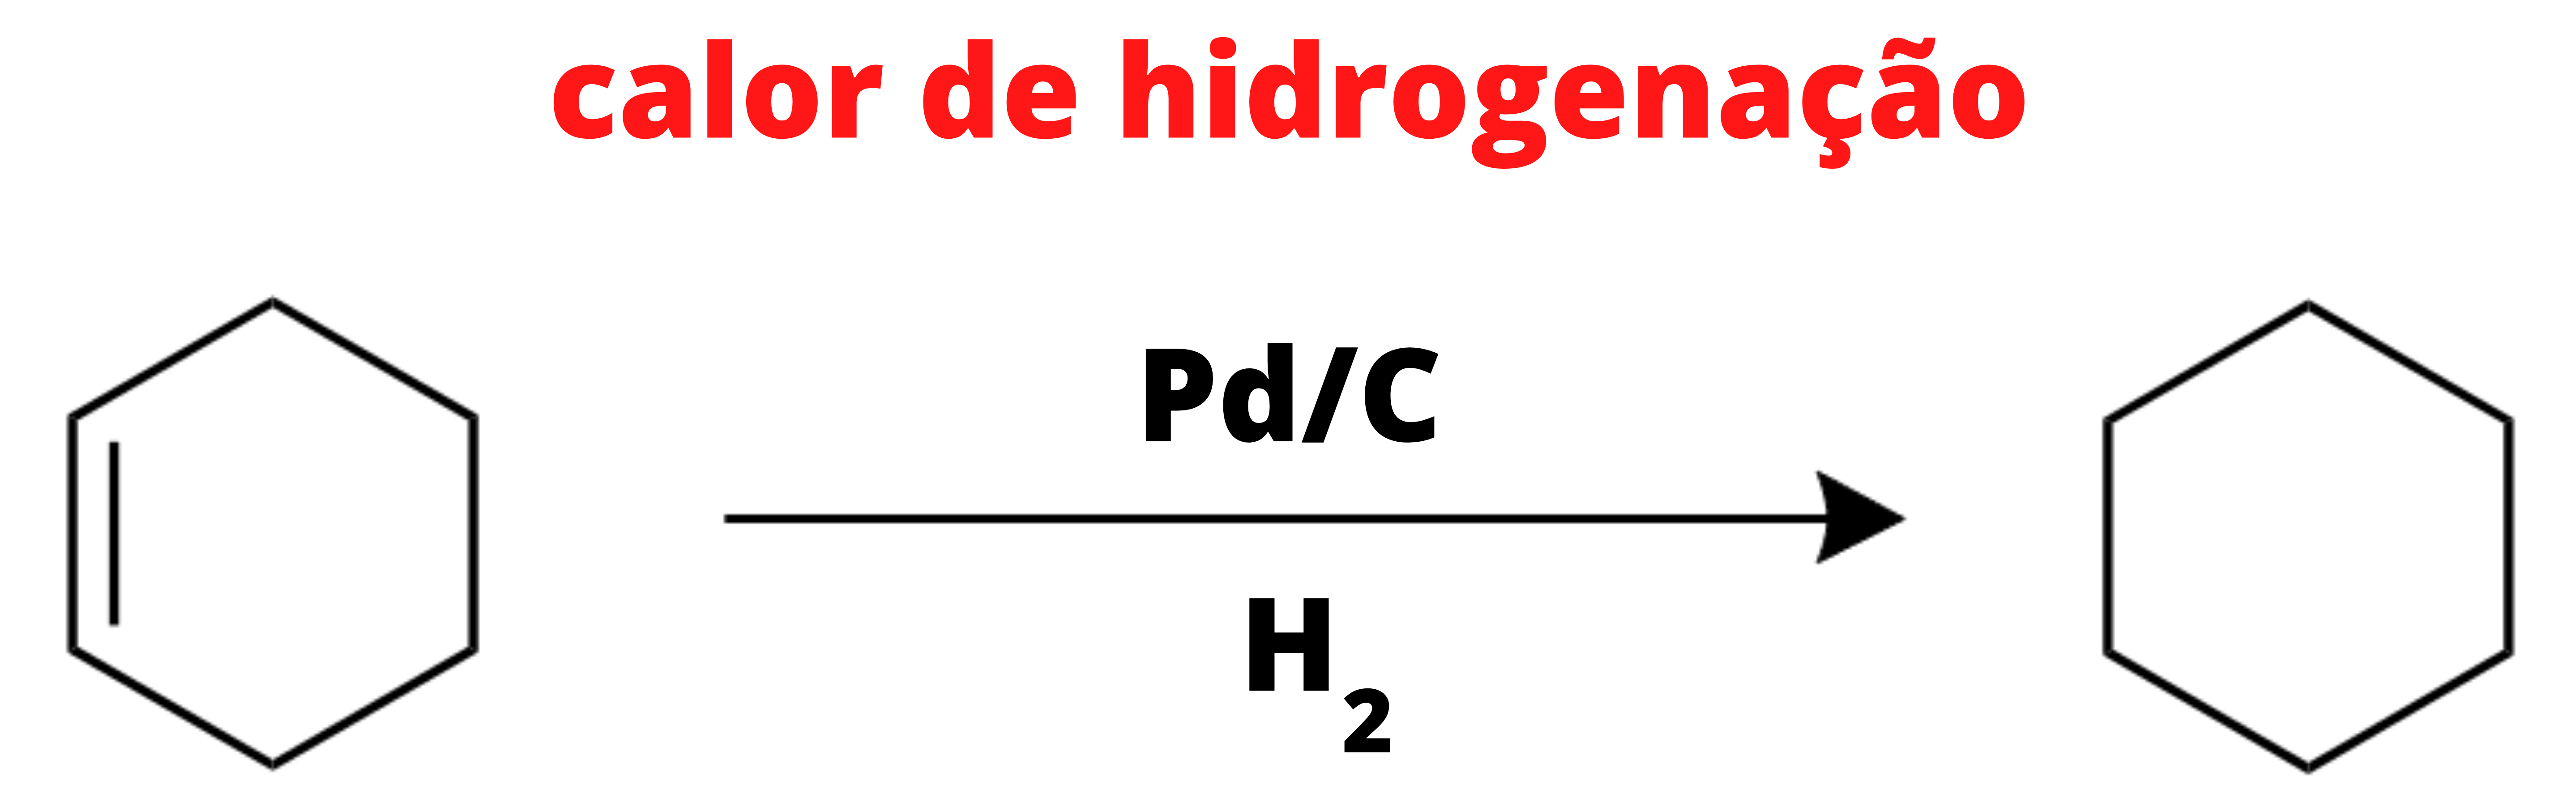
\includegraphics[width=0.5\textwidth]{images/fig1.png}
	\end{center}
	\fonte{Autor(a)}
\end{figure}

Como essa medida é aditiva, se analisarmos o caso do 1,4-cicloexadieno, que possui duas ligações duplas não conjugadas, o calor envolvido no processo será o dobro do que foi observado na situação anterior, isto é, cerca de 56 kcal/mol. No entanto, o isômero conjugado (1,3-cicloexadieno), quando hidrogenado sob as mesmas condições, libera 52,2 kcal/mol (\autoref{fig:2}). A diferença de 3,8 kcal/mol é então chamada de energia de ressonância.

Quando o anel possui três ligações duplas, como na hipótese de um cicloexatrieno, o valor numérico esperado para a entalpia de hidrogenação seria de 85,8 kcal/mol (o triplo do exemplo inicial). Porém, quando essa reação é realizada em condições normais (Pd/C, temperatura ambiente, 1 atm de H$_2$), nada acontece porque o reagente é inerte. Se a pressão for gradualmente aumentada, o cicloexatrieno permanece intacto. Finalmente, submetendo o meio a uma situação drástica (temperatura de 180-220$^\circ$C e 25-30 atm de gás hidrogênio), o reagente hipotético, enfim, gera um cicloexano. Ao medir o calor liberado, o resultado é surpreendente, uma vez que a entalpia obtida é 49,8 kcal/mol, ou seja, 36 kcal/mol abaixo do resultado que era previsto (\autoref{fig:2}). Acontece que o substrato do meio reacional em questão é o benzeno, uma estrutura totalmente conjugada e, por conseguinte, estabilizada pela sobreposição dos orbitais p \autocite{Shaabani2008, Xu2021}. Em função disso, torna-se indispensável a análise comparativa das energias associadas aos orbitais moleculares (MOs), uma vez que o caráter covalente da ligação aumenta, e a diferença de energia entre os orbitais de fronteira diminui quando comparamos as espécies aromáticas e seus análogos sem conjugação.

\begin{figure}[htb]
	\caption{\label{fig:2} Calores de hidrogenação relativos aos hidrocarbonetos cíclicos. Em vermelho, são mostradas as energias de estabilização aromática de cada um dos compostos.}
	\begin{center}
		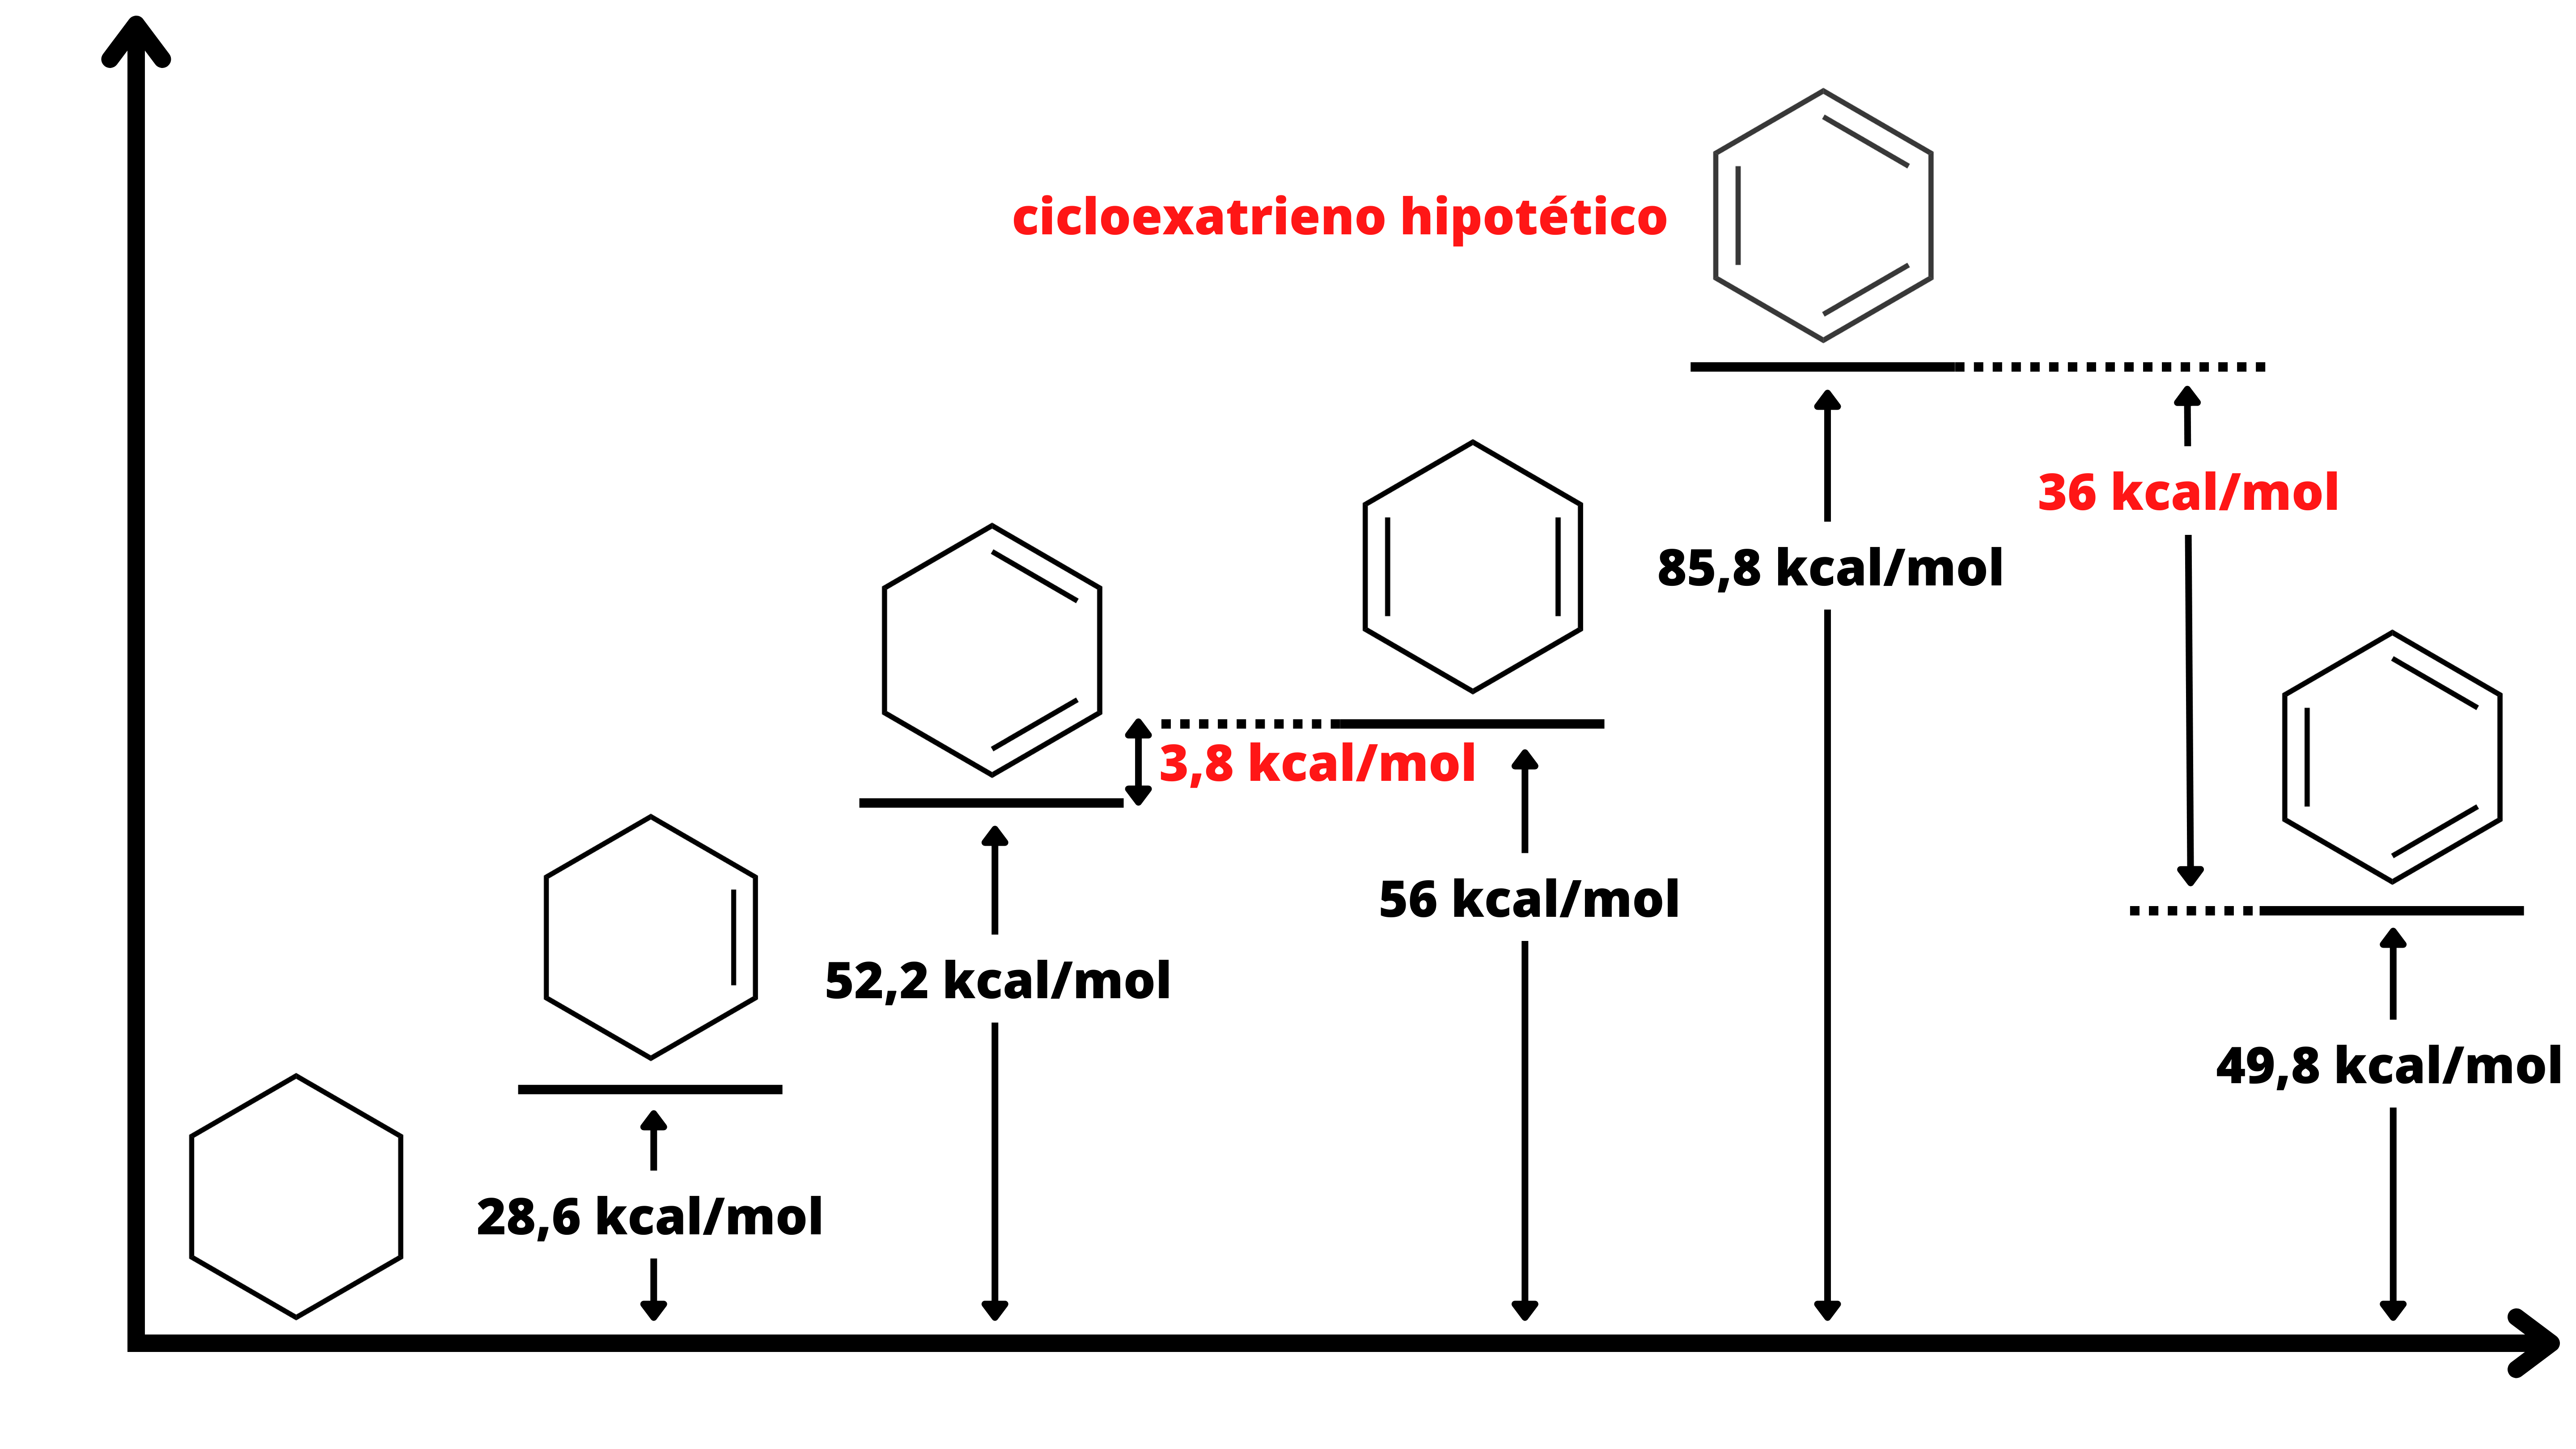
\includegraphics[width=1.0\textwidth]{images/fig2.png}
	\end{center}
	\fonte{Autor(a)}
\end{figure}

%% TODO: falar dos orbitais moleculares de fronteira na aromaticidade.

Como o conceito de aromaticidade é multidimensional\footnote{A multidimensionalidade refere-se ao fato de que o fenômeno da aromaticidade não corresponde, na maioria das vezes, aos mesmos aspectos observados.}, um problema recorrente nessas representações é que um dado critério utilizado para classificar esses compostos não pode, em geral, ser aplicado de maneira consistente. Em muitos casos, encontrar um ponto de referência apropriado é problemático. Por exemplo, os valores de energia de estabilização aromática dependem profundamente dos sistemas de referência em reações virtuais, uma vez que é praticamente impossível deduzir diferenças na aromaticidade de acordo com tendências de reatividade, a menos que sejam consideradas séries de reações estruturalmente similares, a citar, os hidrocarbonetos benzenoides \autocite{Ciesielski2009, Krygowski2014}. Nesse sentido, índices baseados na geometria molecular, tal como \gls{HOMA} \autocite{Kruszewski1972}, também são relativos à escala arbitrária definida previamente.

De acordo com McWeeny, existem também muitas outras noções nos laboratórios de química e nas discussões científicas que podem ser classificadas como padrões fundamentais de entendimento (para além da aromaticidade), pois são lançados mão quase que diariamente para compreender processos químicos de maneira intuitiva. De forma mais específica, podem ser mencionados os termos: confôrmero, nucleófilo, eletrófilo, efeito de solvente, ligações de hidrogênio, acidez/basicidade de Lewis. Para analisar isso mais de perto, e de forma comparativa, foi contabilizado o número de trabalhos científicos por dia que citam alguns desses termos. Os dados mostrados na \autoref{fig:3} foram coletados do a partir de uma busca avançada no \href{https://www-periodicos-capes-gov-br.ez46.periodicos.capes.gov.br/index.php?}{\textit{Portal da Capes}}. É possível notar, através dessa pesquisa, que o tópico da aromaticidade ocupou o topo das pesquisas durante todo o período analisado, com uma média de 60 artigos publicados por dia nos últimos anos do gráfico. 

\begin{figure}[htb]
	\caption{\label{fig:3} Gráfico que relaciona a média de artigos científicos publicados por dia contendo cada um dos termos mostrados na legenda.}
	\begin{center}
		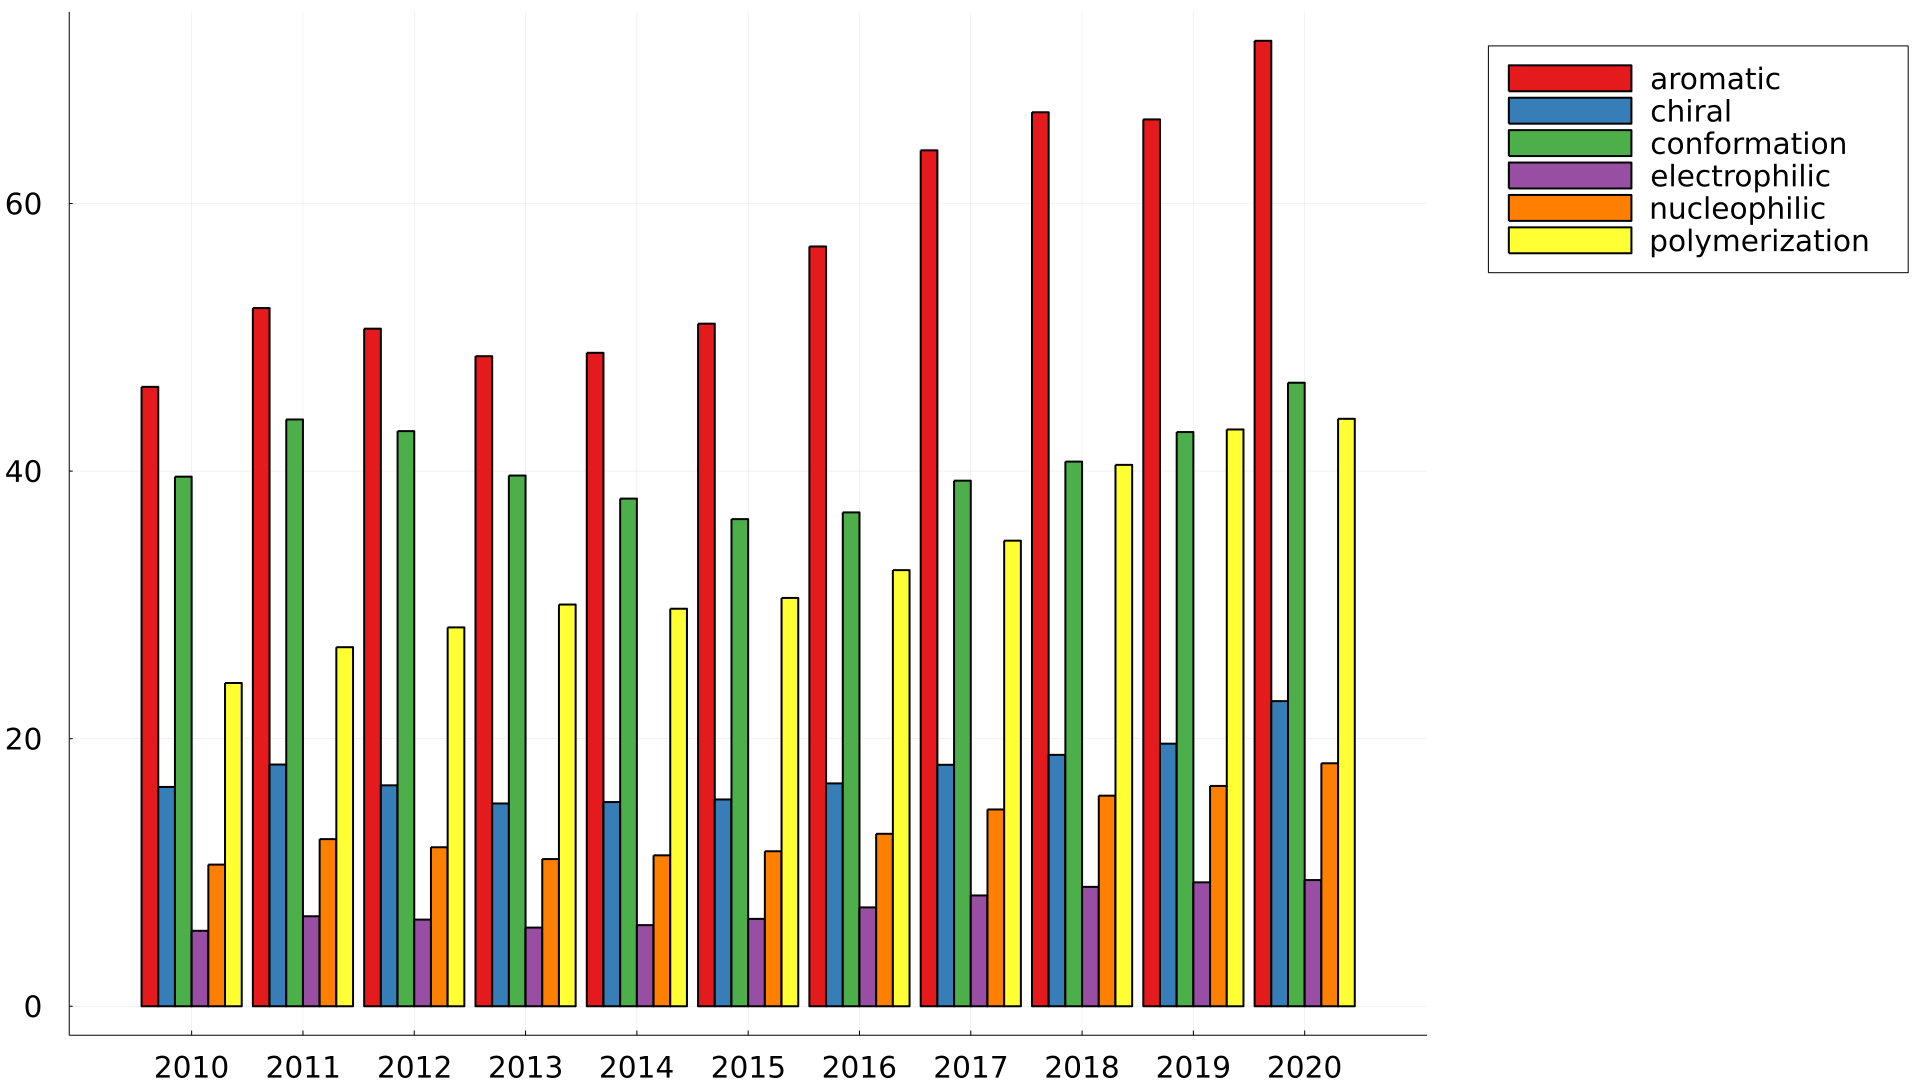
\includegraphics[width=1.0\textwidth]{images/fig3.png}
	\end{center}
	\fonte{Autor(a). Os números são do \href{https://www-periodicos-capes-gov-br.ez46.periodicos.capes.gov.br/index.php?}{\textit{Portal da Capes}}.}
\end{figure}

% Ou seja, a computação gráfica auxilia na manipulação/representação direta dos objetos de estudo químico, sendo eles: átomos, moléculas (leia-se quaisquer agregados atômicos, independentemente da origem de suas interações) ou partes delas. Como esses são elementos de difícil abstração, uma vez que 

% Em tal seguimento, um dos avanços mais importantes é a aplicação da teoria de grafos à notação química e aos sistemas de busca de subestruturas e cálculos de propriedades, como a aromaticidade, que é muito sensível à geometria do sistema $\pi$, pois descreve as moléculas estabilizadas energeticamente pela deslocalização de elétrons móveis em ciclos (geometrias fechadas). Tal temática é extremamente explorada por trabalhos que vem sendo somados desde a primeira citação de Hoffmann na literatura, em 1855. Por exemplo, com uma busca sobre os termos aromático/aromaticidade no \textit{\href{https://scholar.google.com.br/scholar?hl=pt-BR&as_sdt=0\%2C5&as_ylo=2016&as_yhi=2022&q=aromatic&btnG=}{Google Scholar}} no período de 2016 a 2022, foram encontrados mais de 380 trabalhos/dia publicados, sendo a maioria destes na área de Química, uma vez que, entre os compostos carbocíclicos, destacam-se os derivados aromáticos, cuja estabilidade e reatividade dependem do caráter de deslocalização eletrônica. Para tais sistemas, é possível utilizar a equalização dos comprimentos de ligação como principal critério geométrico de análise quantitativa.


O presente trabalho pretende, fundamentado nesse conjunto de informações, relacionar as propriedades extraídas das representações moleculares a partir da computação gráfica, produzindo uma interface para manipular esses compostos de forma facilitada e didática. Uma vez que as dificuldades de compreensão por parte dos graduandos em relação aos conceitos e fenômenos originam-se na forma com que são apresentados \autocite{Cunha2018}, a ferramenta proposta poderá ser difundida para uso didático-pedagógico, podendo ser utilizada por discentes e docentes durante as aulas no sentido de demonstrar os modelos de classificação e a multidimensionalidade da aromaticidade, facilitando o entendimento. O nome atribuído a tal ferramenta foi \textit{Balmy.jl}. A extensão (\textit{.jl}) junto ao nome testifica que o \textit{software} foi produzido na linguagem Julia; e o termo \textit{Balmy}, de origem inglesa, faz alusão ao primeiro critério qualitativo de classificação dos compostos aromáticos: o odor, resgatando a historicidade do conceito de forma criativa.

% Assim, usuário será capaz de calcular os parâmetros geométricos de aromaticidade, um conceito explorado de forma superficial e pouco visual dentro das salas de aula. 

% ----------------------------------------------------------
\chapter{Revisão Bibliográfica}
% ----------------------------------------------------------

Historicamente, as primeiras evidências do uso da terminologia \textit{aromática(o)} remontam ao ano de 1800, mais especificamente à classificação qualitativa\footnote{Importante ressaltar que a noção de \textit{classificação qualitativa} citada pelo trabalho refere-se ao fato de, na época, não se ter conhecimento da estrutura química desses compostos.} de substâncias e óleos essenciais oriundos de produtos naturais através do odor, a exemplo da vanilina e do anetol. Nada obstante, tal ideia caiu em desuso por conduzir, mesmo na época, a associações espúrias como no caso do (-)-mentol.

Décadas depois (1825), Michael Faraday\autocite{Faraday1925, Wilson2012, Martin2015} conseguiu isolar pela primeira vez o benzeno\footnote{O nome do benzeno é derivado do ácido benzoico, descoberto no século XVI. O ácido foi assim designado por ter sido obtido pela destilação seca da goma de benjoim, uma planta nativa da Sumatra, descrita pela primeira ver por Nostradamus em 1555, depois por Aleixo Pedemontanus em 1560 e, em seguida, por Blaise de Vinagère, no ano de 1596}, um hidrocarboneto aromático com alto grau de toxicidade associado\autocite{Solomon1977}. Esse produto foi obtido por fracionamento repetido do fluido obtido durante a compressão do gás petrolífero (o acetileno, usado na iluminação das ruas de Londres, e produzido através da pirólise do óleo de baleia) fornecido através da bondade do Sr. Gordon da \href{https://portablegas.co.uk/}{\textit{Portable Gas Company}}. Ele deduziu que a fórmula molecular do composto obtido correspondia ao "bicarbureto de hidrogênio" (\ce{C_6H_3}), baseado na massa do hidrogênio, que na época era incorreta. No entanto, ele determinou o ponto de ebulição associado ao produto final, além da sua densidade, com certa acurácia e, ao comparar seus dados com aqueles retidos do \textit{trans}-2-buteno, o qual Faraday também isolou, notou que era muito mais reativo do que o benzeno. Esse episódio representa um marco extremamente significativo para a construção da ideia de aromaticidade, uma vez que o benzeno é inegavelmente o composto mais famoso dessa classe de moléculas com propriedades derivadas da deslocalização de elétrons $\pi$\autocite{Faraday1825}. 

Poucos anos depois, em 1834, Eilhard Mitscherlich também realizou a síntese do benzeno, mas agora partindo do ácido benzoico. Esse processo ocorre sob aquecimento na presença de cal virgem (\ce{CaO}), produzindo o benzeno como destilado do meio reacional e calcário (\ce{CaCO_3}). Uma alternativa foi proposta por Mansfield (1845), que isolou o benzeno a partir do alcatrão de hulha sob um procedimento que \textit{a posteriori} foi adaptado à indústria. Apesar da fórmula molecular \ce{C_6H_6} já ser conhecida em meados do século XIX, restavam muitas dúvidas sobre os aspectos estruturais do benzeno, uma vez que essa era uma área em defasagem na época. 

A partir de 1860 os químicos estruturalistas; como Loschimidt (1861) Laderburg (1869), Claus (1866) e Dewar (1866), começaram a intencionar hipóteses sobre a estrutura do benzeno, até chegar, em 1865, na proposta de Kekulé, que se assemelha mais ao que seria a real representação estrutural do composto, fato que só foi devidamente reconhecido décadas mais tarde (1890) e comprovado em 1929\autocite{Lonsdale1929}, com a obtenção da primeira estrutura de raios-X de um derivado, o hexametilbenzeno. A base que sustenta até hoje esse modelo foi relatada inicialmente em todo o seu trabalho envolvendo os ácidos benzóico e salicílico, de ordem crucial para o avenço de diversos conceitos químicos.

Com a virada do século XIX para o XX, passou-se a ganhar entendimento da inexistência de um equilíbrio formal entre as formas isoláveis do benzeno, mas sim das estruturas canônicas de ressonância que perfazem um híbrido com elétrons móveis através de um efeito isomérico chamado mesomeria \autocite{Murrell1956, INGOLD1934, Oudar1975}. Os compostos insaturados aromáticos possuem, também, propriedades aditivas inerentes aos átomos e ligações que os constituem, como a exaltação da susceptibilidade magnética\autocite{Schleyer1996, Schleyer2001, Schleyer2014}. Segundo Pascal (1910) no artigo intitulado \textit{Magnetochemical researches}\autocite{pascal1910magnetochemical}, a mobilidade eletrônica em estruturas cujas ligações duplas são alternadas torna-as diamagnéticas, isto é, não possuem magnetização a campo zero e apresentam uma magnetização contrária quando um campo é aplicado. Por isso, os compostos aromáticos são capazes de induzir campos magnéticos significativos a ponto de interferir nas frequências de ressonância de átomos ligados ao anel aromático. Neste caso, são conhecidos os efeitos de proteção e desproteção de núcleos provocados pelas correntes de anel.

Foi então no ano de 1931, quando a fundamentação estrutural da aromaticidade se tornava mais sólida, que surgiu uma das primeiras regras de classificação de moléculas aromáticas desenvolvida por Erich Hueckel\autocite{Hckel1931}. Utilizando a teoria dos orbitais moleculares, ele elucidou muitos pontos sobre as propriedades eletrônicas de compostos orgânicos, o que o permitiu demonstrar que hidrocarbonetos cíclicos com ($4n+2$) elétrons $\pi$ (sendo $n$ um número inteiro) possuem um incremento da estabilidade energética. Hueckel\autocite{Hckel1931, Brogli1972} justificou este efeito através da distribuição eletrônica dos compostos aromáticos, uma vez que, para ele, a razão do abaixamento da energia dos compostos aromáticos devia-se à ausência de elétrons desemparelhados.

Tal abordagem tem, no entanto, suas excepcionalidades, a exemplo dos [10]anulenos, que possuem o número adequado de elétrons $\pi$, mas não as demais propriedades associadas à aromaticidade (estabilidade, reatividade, propriedades magnéticas típicas e planaridade da molécula). Essa distorção é causada por fatores topológicos e efeitos estereoeletrônicos observados nesses compostos, pois os hidrogênios internos das estruturas dos [10]anulenos afetam boa conjugação do sistema $\pi$ \autocite{Caramori2006}. 

Simultaneamente, surgiram algumas estratégias experimentais para a determinação das energias de ressonância, que justificam o aumento da estabilidade dos compostos aromáticos. Pauling (1933) \autocite{Pauling1933, Pauling1936} e Kistiakowsky (1936) calcularam a energia de ressonância do benzeno baseando-se nos calores de hidrogenação ($\Delta H^{\circ}_{\textit{hidrogenação}}$) de algumas reações selecionadas. Eles encontraram valores em torno de 36 kcal/mol, o que serviu para comparar com os parâmetros já conhecidos para alcenos não conjugados e assim aprofundar o estudo físico-químico da aromaticidade. Dessa forma, com o avanço da química quântica e dos métodos teóricos de análise dos arranjos atômicos no século XX, evoluíram também os critérios para se avaliar se os compostos podem ser classificados como:

\begin{enumerate}
    \item \textit{aromáticos} (estabilizados por ressonância de elétrons);
    \item \textit{não-aromáticos} (não sofrem efeito mesomérico);
    \item \textit{antiaromáticos} (desestabilizados por efeitos geométricos, torcionais e estereoeletrônicos); quais sejam, de origem geométrica, magnética e energética. 
\end{enumerate}

\section{Critérios Geométricos}

Os critérios geométricos são aplicados não somente à molécula inteira, como nos outros critérios, mas também podem ser utilizados para estudar fragmentos de sistemas $\pi$-eletrônicos cíclicos ou não. Os indicadores NICS pode, por sua vez, ser aplicados aos anéis individualmente (dependendo do tamanho do ciclo em questão). Em quase todos os casos considerados, os índices geométricos descrevem o grau de elétrons-$\pi$ ou deslocalização de ligações duplas. A natureza da equalização dos comprimentos de ligação dupla é amplamente investigada, mas aqui, aceitamos o pressuposto de que ela é advinda da deslocalização eletrônica.

Ou seja, os índices geométricos de aromaticidade, servem para três propósitos:

\begin{enumerate}
    \item estimar o caráter aromático de uma dada molécula em comparação a outras;
    \item testar novas características numéricas por análises estatísticas de similaridade com outros índices;
    \item estudar as mudanças na aromaticidade devido às perturbações intra- ou intermoleculares.
\end{enumerate}

\subsection{O conceito de Julg Aj (1967)}



% ----------------------------------------------------------
\chapter{Objetivos}
% ----------------------------------------------------------

% ----------------------------------------------------------
\section{Objetivo Geral}
% ----------------------------------------------------------

 Desenvolver um \textit{software} de interação gráfica capaz de representar a molécula tridimensionalmente através da leitura de dados de coordenadas cartesianas atômicas e assim retornar parâmetros de aromaticidade segundo a metodologia definida pelo usuário. Poderá, portanto, ser utilizado como uma ferramenta de pós-processamento para o cálculo de propriedades eletrônicas. Além disso, também pretende-se implementar métodos semiempíricos de baixo custo computacional (Hueckel e Hueckel estendido) para auxiliar na avaliação e representação dos orbitais atômicos e moleculares.

% ----------------------------------------------------------
\section{Objetivos Específicos}
% ----------------------------------------------------------

\begin{itemize}
    %\item Realizar pré-otimizações de geometria utilizando métodos semi-empíricos e \textcolor{red}{realizando leituras de estruturas obtidas por outros métodos através de outros \textit{softwares}; complementar};
    
    \item Utilizar métodos semiempíricos para avaliar orbitais atômicos e moleculares.
    
    \item Automatizar a leitura de arquivos de saída \textit{outputs} \textit{logfiles} de cálculos de estrutura eletrônica molecular visando extrair dados geométricos para determinar critérios de aromaticidade geométricos em sistemas orgânicos, através de uma interface gráfica.

    \item Utilizar a teoria de grafos para implementar a determinação dos índices HOMA, EN, e GEO; 
    
    \item Realizar \textit{benchmark} dos resultados obtidos com estruturas já reportadas na literatura para fins de  validação e comparação do tempo de computação na metodologia aplicada.
\end{itemize}